%
% 1-frueh.tex
%
% (c) 2026 Prof Dr Andreas Müller
%
\section{Die frühe Entwicklung der Analysis
\label{buch:einleitung:section:frueh}}
\kopfrechts{Die frühe Entwicklung der Analysis}

\subsection{Frühe Vorläufer
\label{buch:einleitung:frueh:subsection:vorlaeufer}}
%
% fig-parabel.tex
%
% (c) 2026 Prof Dr Andreas Müller
%
\begin{figure}
\centering
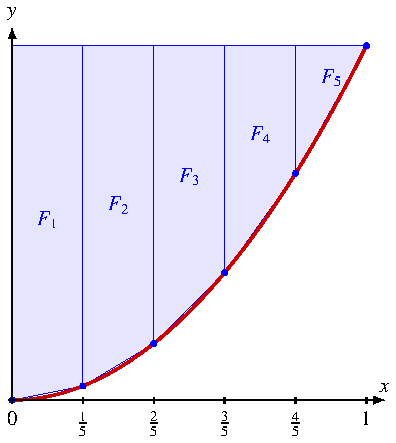
\includegraphics{chapters/000-einleitung/images/parabel.pdf}
\caption{Exhaustion der Parabel $y=x^2$
\label{buch:einleitung:fig:parabel}}
\end{figure}
%
Schon Archimedes war in der Lage, den Flächeninhalt eines
Parabelbogens zu bestimmen.
\index{Archimedes}%
\index{Parabelbogen}%
Mit seiner Methode der Exhaustion approximierte er durch Polygone,
\index{Exhaustion}%
deren Flächeninhalt mit rein algebraischen Methoden bestimmt werden
konnte.
Durch feiner werdende Unterteilung der Polygone konnte eine beliebig
genaue Näherung gefunden werden.
Den Parabelbogen $y=x^2$ mit $x\in [0,1]$ (siehe
Abbildung~\ref{buch:einleitung:fig:parabel}) kann man z.~B.~durch Unterteilung
in $n$ Stützstellen $x_i = \frac{i}{n}$, $i=0,\dots,n$, als Vereinigung
von Trapezen mit jeweils dem Flächeninhalt
\begin{align*}
|F_i|
&=
\frac12 \biggl(
\biggl( 1-\frac{(i-1)^2}{n^2} \biggr)
+
\biggl( 1-\frac{i^2}{n^2} \biggr)
\biggr)
\cdot
\frac{1}{n}
\\
&=
\frac1{2n^3}\bigl(
n^2-(i-1)^2+n^2-i^2
\bigr)
=
\frac1{2n^3}\bigl(
2n^2
-1+2i-2i^2
\bigr)
\end{align*}
betrachten.
Die Summe dieser Flächen ist
\begin{align}
F(n)
&=
\sum_{i=1}^n
F_i
=
\sum_{i=1}^n
\frac1{2n^3}
\bigl(
2n^2
-1+2i-2i^2
\bigr)
\notag
\\
&=
\frac1{2n^3}
\sum_{i=1}^n
\bigl(
2n^2
-1+2i-2i^2
\bigr)
=
1
-
\frac1{2n^3}
\biggl(
-
\sum_{i=1}^n 1
+
2
\sum_{i=1}^n i
-
2
\sum_{i=1}^n i^2
\biggr).
\notag
\intertext{Für die einzelnen Summen sind algebraische Ausdrücke in $n$
bekannt, sie ergeben}
&=
1
-
\frac1{2n^3}
\biggl(
-
n
+
2
\frac{n(n+1)}2
-
2
\frac{n(n+1)(2n+1)}{6}
\biggr)
\notag
\intertext{oder ausmultipliziert}
&=
1
-
\frac1{6n^3}
\bigl(
-
3
n
+
3n^2+3n
-
(n+3n^2+2n^3)
\bigr)
\notag
\intertext{und zusammengefasst}
&=
1
-
\frac1{6n^3}
\biggl(
-
n
+
2n^3
\biggr)
=
1-\frac{1}{3}
-\frac{1}{6n^2}
=
\frac23
-\frac{1}{6n^2}.
\label{buch:einleitung:frueh:eqn:summen}
\end{align}
Damit sind die algebraischen Umformungen abgeschlossen.
Jetzt wird argumentiert, dass für grosse $n$ die letzten zwei Terme
von \eqref{buch:einleitung:frueh:eqn:summen}
nur einen sehr kleinen Beitrag zur Fläche leisten, im Grenzwert
verschwinden und daher die Fläche
\[
\lim_{n\to\infty} F(n) = \frac23
\]
ist.

Die Exhaustionsmethode findet algebraische Ausdrücke für den
Flächeninhalt $F(n)$ in Abhängigkeit von der Anzahl $n$ Teilpolygone
und bestimmt ad hoc den Grenzwert für $n\to\infty$.
Mit dieser Methode konnte Archimedes auch eine Abschätzung der
Kreiszahl $\pi$ geben.

%
% Newtons Fluxionen
%
\subsection{Newtons Fluxionen
\label{buch:einleitung:frueh:subsection:newton}}
Newton wurde zur Entwicklung seiner Form der Infinitesimalrechnung
motiviert durch die Beschreibung mechanischer Vorgänge.
\emph{Fluenten} sind in seiner Terminologie Grössen, die sich mit der
Zeit ändern können.
Heute würden wir sagen: Fluenten sind Funktionen der Zeit.
\index{Fluente}%
Die Idee einer Funktion war schon vor Newton bekannt.
\index{Newton, Isaac}%
Nicolaus von Oresme hat sich die Methode erdacht, die Abhängigkeit
\index{Oresme, Nikolaus von}%
von Grössen durch einen Graphen zu visualisieren und diesen als
Werkzeug für die Untersuchung zu verwenden.
In seinem Werk findet man auch die Idee, Flächen und Volumina in
Streifen oder Quader zu zerlegen und so der Berechnung ähnlich
der Exhaustionsmethode zugänglich zu machen.

Die instante Änderungsrate einer Fluenten wird \emph{Fluxion} genannt.
\index{Fluxion}%
Die Fluxion der Fluente $x(t)$ wird mit $\dot{x}(t)$ bezeichnet.
Ohne bereits im Besitz eines Grenzwertbegriffs zu sein, entwickelt
er auch Methoden zur Berechnung von Fluxionen für Funktionsterme, die
die Zeit $t$ als Parameter enthalten.
Solche algebraischen Regeln zur Berechnung der Ableitungen machen
den Erfolg der Methode aus.

Newton erkannte auch, dass es möglich ist, von der Fluxion wieder
zurück zur Fluenten zu gelangen.
Seine Notation für diese Operation war uneinheitlich, er hat sowohl
die Zeichen $\bar{x}$ wie auch $\boxed{x}$ verwendet.
Dies hat letztendlich die Anwendung seiner Methode erschwert und
dazu geführt, dass heute fast ausschliesslich die von Leibniz
eingeführte Notation verwendet wird.
Abgesehen von der schwierigen Notation von Newtons Technik kann man sagen,
dass Newton auch der Hauptsatz der Infinitesimalrechnung bereits bekannt war.

%
% Die Notation von Leibniz
%
\subsection{Die Notation von Leibniz
\label{buch:einleitung:frueh:subsection:leibniz}}
Leibniz hat seine Ideen zur Infinitesimalrechnung unabhängig von Newton
\index{Leibniz, Gottfried Wilhelm}%
und unabhängig von der unmittelbaren physikalischen Anwendung
entwickelt.
Newton war ihm zwar zuvorgekommen, doch hat dieser sein Methode erst
viel später veröffentlicht.
Leider entbrannte später auch ein heftiger Prioritätsstreit zwischen
Newton und Leibniz.
\index{Prioritatsstreit@Prioritätsstreit}%

Unabhängig von der Frage der Priorität ist es das besondere Verdienst
von Leibniz, eine intuitiv zugängliche Notation gefunden zu haben,
die noch heute gelehrt wird und die Basis von Erweiterungen ist.
Die Ableitung ist motiviert durch die Sekantensteigung eines
\index{Sekante}%
\index{Steigung}%
Funktionsgraphen $y=f(x)$, die durch den Differenzenquotienten
\[
\frac{\Delta y}{\Delta x}
=
\frac{f(x+\Delta x) - f(x)}{\Delta x}
\]
berechnet wird.
Leibniz hat sich vorgestellt, die endliche Grösse $\Delta x$ durch
ein infinitesimale Grösse $dx$ zu ersetzen, was ihn auf die Notation
\[
\frac{dy}{dx}
=
\frac{d}{dx}f(x)
=
\lim_{\Delta x\to 0}
\frac{f(x+\Delta x) - f(x)}{\Delta x}
\]
geführt hat.
Newtons Fluxion einer Fluenten $x(t)$ wird in dieser Notation
als
\[
\dot{x}(t) = \frac{dx}{dt}
\]
geschrieben.

Für ein Zusammensetzung $f(g(x))$ ist die Ableitung in der leibnizschen
Notation 
\[
\frac{d}{dx}f(g(x))
=
\frac{df}{dg}\cdot \frac{dg}{dx}
=
\frac{df}{dx}(g(x))\cdot \frac{dg}{dx}(x).
\]
Die Kettenregel, die auch Newton schon bekannt war, erhält so die
\index{Kettenregel}%
intuitive algebraische Form einer Kürzungsregel.
\index{Kurzungsregel@Kürzungsregel}%

Für das Integral erfand Leibniz die Notation des Integralzeichens.
\index{Integralzeichen}%
\index{S@$\int$}%
Die Fläche unter einem Funktionsgraphen stellte er sich als die
Vereinigung von Rechtecken der Höhe $f(x)$ und der Breite $\Delta x$
vor, deren Inhalt sich zu
\[
\sum f(x)\,\Delta x
\]
summiert.
Um den exakten Wert des Flächeninhalts unter der Kurve zu bestimmen,
ersetzt er die endliche Breite $\Delta x$ eines Streifens durch die
infinitesimale Breite $dx$ und die endliche Summe $\sum$ durch eine
``unendliche Summe'' und schreibt
\[
F
=
\int_a^b f(x)\,dx
\]
für den Flächeninhalt unter der Kurve $y=f(x)$ zwischen den $x$-Werten
$a$ und $b$.

Auch Leibniz erkannte, dass die Integration die Umkehroperation zur
Differentiation ist.
In seiner Notation lautet der Hauptsatz der Infinitesimalrechung
\index{Hauptsatz der Infinitesimalrechnung}%
\[
\int_a^b \frac{df}{dx}\,dx
=
\int df
=
f(b) - f(a),
\]
auch hier erlaubt die leibnizsche Notation ein natürliche Interpretation.

